\chapter{Vývoj}
\label{chap:development}

V této kapitole je popsána celková implementace modelové hry, která byla vytvořena na základě stanovených požadavků a návrhu herního systému, popsaných v předchozích kapitolách.

Hybridní deskové hře, která je finálním produktem této práce, bylo určeno pracovní jméno \textit{Trails Through Shadows} (zkratkou \textit{TTS}). I nadále však bude zmiňována především pod názvem \textit{modelová hra}. Dále je důležité zmínit, že veškerý text, který je součástí modelové hry, je napsán v angličtině.

\section{Spolupráce}
\label{sec:collaboration}

Deskové hry, především ty hybridní, mohou být velmi komplexní a náročné na vývoj. Proto byla spolupráce specifikována přímo v samotném zadání a řešení bylo realizováno v týmu čtyř studentů.

\subsection{Rozdělení práce}
\label{subsec:job_distribution}

\begin{figure}[h]
    \centering
    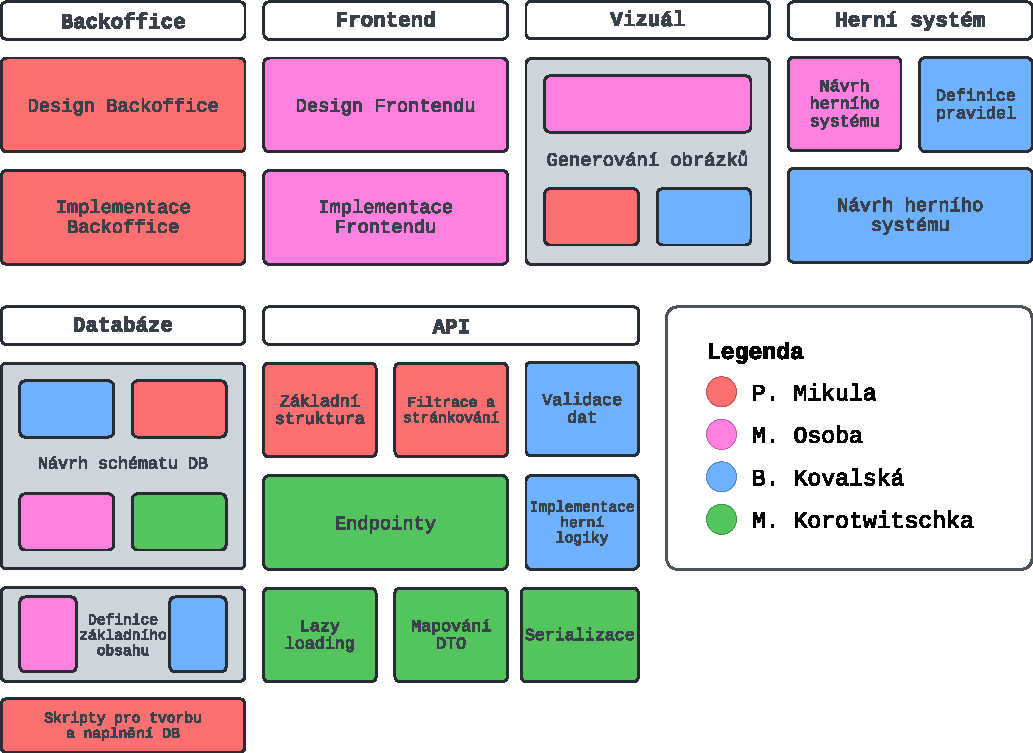
\includegraphics[width=\textwidth]{../../shared/diagrams/blocks.pdf}
    \caption{Rozložení práce v týmu}
    \label{fig:job_distribution}
\end{figure}

Hlavními čtyřmi částmi projektu byla tvorba \textbf{administrativního rozhraní} (Pavel Mikula), \textbf{uživatelského prostředí} (Miroslav Osoba), \textbf{API} (Martin Korotwitschka) a konečně implementace \textbf{herního modelu} (Barbora Kovalská), která je tématem této práce. Samotné vypracování však nebylo nutně omezeno pouze na tyto části, a tak se v průběhu vývoje mohlo stát, že se členové týmu podíleli i na jiných částech projektu.

Rozvržení práce vyobrazeno na obrázku \ref{fig:job_distribution} bylo provedeno především s ohledem na zájmy a schopnosti jednotlivých členů týmu, podle čehož se také v prvé řadě přidělovalo samotné zadání bakalářské práce. V samotném grafu byly tyto části rozděleny do bloků a rozšířeny ještě o dvě další sekce, které se ukázaly být dostatečně velké na to, aby se od ostatních osamostatnily -- \textbf{databáze} a \textbf{vizuální vzhled} hry. 

Jednotlivé bloky znázorňují určitou část dané sekce, přičemž velikost daného bloku reprezentuje mohutnost tohoto úkolu. Dílčí části, na kterých se podílelo více členů týmu, jsou reprezentovány šedě s barevnými bloky, jejichž velikost opět znázorňuje poměr práce jednotlivých spoluřešitelů.

Části projektu, na kterých se pracovalo v této práci, budou popsány v následujících sekcích.

\subsection{Organizace projektu}
\label{subsec:versioning}

\begin{figure}[h]
    \centering
    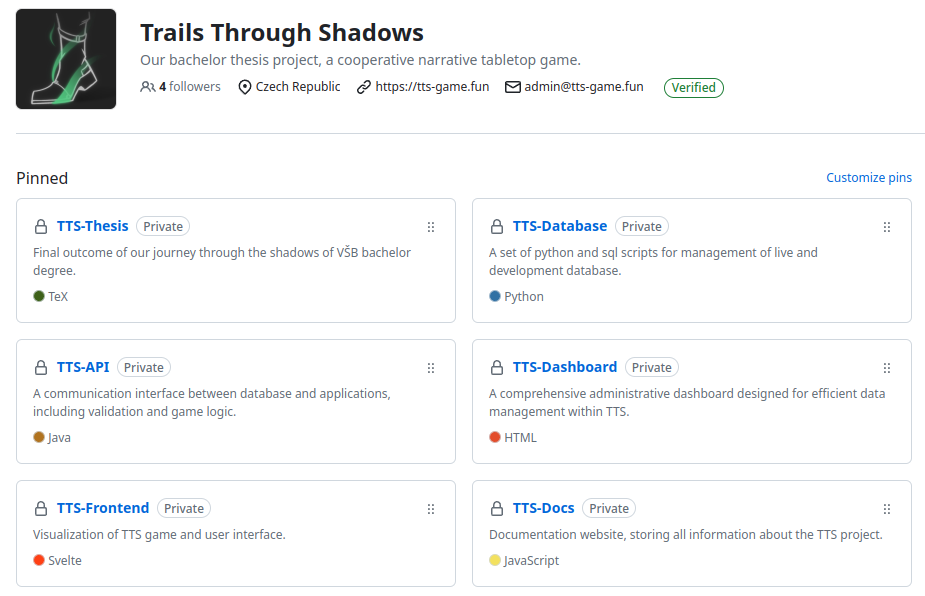
\includegraphics[width=\textwidth]{../../shared/figures/gitOrg.png}
    \caption{Rozdělení repozitářů v rámci organizace}
    \label{fig:git_organization}
\end{figure}

Pro ucelení vývoje a zajištění efektivní spolupráce byla v rámci implementace vytvořena organizace \devTool{Trails Through Shadows}{https://github.com/Trails-Through-Shadows} na platformě \devTool{GitHub}{https://github.com}, kde byly vytvořeny repozitáře pro jednotlivé části projektu, jak je možné vidět na obrázku \ref{fig:git_organization}. Organizace byla opatřena logem, které bylo vytvořeno v rámci zadání práce a bylo použito i pro další potřeby týmu.

\begin{description}
    \item [TTS-Dashboard] -- Administrativní rozhraní, sloužící ke správě hry, jednotlivých lokací, nepřátel a dalších entit. Primární použití je pro vývojáře, kteří zde mohou vytvářet a upravovat herní obsah.
    \item [TTS-Frontend] -- Uživatelské prostředí, které slouží k interakci se hrou. Hráči zde mohou vidět své rozehrané kampaně a postavy a také vizualizaci celého souboje včetně herní mapy, iniciativního žebříčku a nepřátel.
    \item [TTS-Api] -- API, umožňující strukturovanou komunikaci mezi databází a jednotlivými částmi hry. Obsahuje nejen základní CRUD funkcionalitu, ale i další metody pro komunikaci, autentizaci a autorizaci, validaci vstupních dat a také implementaci samotného herního systému pro správný chod hráčského prostředí.
    \item [TTS-Database] -- Nejedná se o databázi jako takovou, neboť ta je hostována na serveru, ale o skripty pro její vytvoření a naplnění výchozích dat.
    \item [TTS-Docs] -- Dokumentace projektu, taktéž hostována na serveru, která obsahuje dokumentaci, jež je vytvářena v průběhu vývoje.
    \item [TTS-Thesis] -- Repozitář pro bakalářskou práci, který obsahuje veškeré zdrojové kódy a soubory potřebné pro vygenerování této práce. Každý z členů týmu zde má svou vlastní složku, kde se nachází zdrojové kódy \LaTeX{u} jeho dokumentu, a také je zde složka \texttt{shared}, která obsahuje společné soubory, jako jsou obrázky a diagramy týkající se sdílených částí projektu. 
\end{description}

Spolu s organizací byla také zakoupena doména \texttt{tts-game.fun}, na kterou byly nasazeny veškeré části projektu, u kterých to bylo přínosné. Kontinuální integrace byla prováděna při každém commitu do hlavní větve repozitáře, kde byl vytvořen nový build a následně byl nasazen na server. Tento systém byl zajištěn pomocí služby \devTool{GitHub Actions}{https://github.com/features/actions} a umožňoval všem členům týmu vidět aktuální stav projektu a jeho vývoj.

Pro zvýšení přehlednosti a efektivity souběžného vývoje tým využíval \devTool{Github Issues}{https://github.com/features/issues}, kde byly vytvářeny úkoly, které bylo možné přiřadit jednotlivým členům týmu. Co se týče větví, byl využit systém \texttt{master} - \texttt{development} - \texttt{feature}, pro úkoly tedy byla vytvořena feature branch, kde byly prováděny změny a po dokončení byl vytvořen pull request do developmentu, který byl po schválení sloučen i do hlavní větve.


\section{Implementace}
\label{sec:implementation}

Hlavním řešenou oblastí byla samotná implementace herního modelu, který byl základem celé hry, ale jak je možné vidět z diagramu \ref{fig:job_distribution}, během vývoje vznikla potřeba řešit i menší dílčí části. Tato sekce se zaměřuje na poznatky a problémy, které byly řešeny v průběhu vývoje.

\subsection{Databáze}
\label{subsec:database}

Návrh databáze byl vysvětlen v kapitole \ref{sec:design_scheme}, kde byly popsány jednotlivé entity a vztahy mezi nimi. Pro zjednodušení vývoje byl využit nástroj \devTool{dbdiagram}{https://dbdiagram.io/home}, který umožňuje vytvářet a vizualizovat schémata databází a následně je exportovat do souboru, který je možné použít pro skripty k jejímu vytvoření. Pro implementaci byla zvolena databáze \devTool{MariaDB Server}{https://mariadb.org/}, která byla hostována na serveru a byla přístupná primárně pomocí \textit{API}.

Na tvorbě návrhu se podíleli všichni členové týmu, kteří měli možnost navrhovat a upravovat schéma databáze, a také byli schopni vytvářet a upravovat data v databázi. Samotný návrh se v průběhu vývoje měnil, a to především kvůli změnám v herním modelu, které byly zjištěny až při implementaci. O případných změnách byli vždy všichni členové informováni včas a u těch s většími zásahy se vedla diskuze, zda je změna nutná a jaký bude její dopad na zbytek projektu. Pro testovací účely vznikla také vývojová databáze \textit{tts\_api\_dev}, kde byly testovány nové změny před nasazením na produkci \textit{tts\_api}.

V rámci práce na projektu bylo také třeba definovat výchozí data, která dávala smysl jak z herního hlediska, tak i z hlediska testování. Tento úkol byl svěřen těm členům týmu, kteří měli největší znalost herního modelu a byli schopni vytvořit data, která byla pro testování dostačující. Pro začátek bylo tedy vytvořeno několik lokací, nepřátel a čtyři rasy a třídy, každá se svými jedinečnými akcemi a efekty, které byly dostatečné pro testování základních funkcí hry. Data se do databáze vkládala pomocí skriptů napsaných v jazyce \devTool{Python}{https://www.python.org/}, které jako vstup přijímaly soubory ve formátu \texttt{JSON} a následně je vkládaly do databáze.

\subsection{Vizuál hry}
\label{subsec:game_visuals}

Na vizuální stránce hry se podílel především člen týmu zodpovědný za uživatelské rozhraní, jisté úkoly, především tvorba obrázků, zde však byly delegovány i na jiné členy týmu. Pro vytvoření vizuálně atraktivní hry bylo třeba vytvořit obrázky pro lokace, předměty, nepřátele, rasy a třídy, a také pro každou kombinaci, která může vzniknout při tvorbě postavy. V rámci vývoje bylo rozhodnuto o použití generátoru \devTool{Midjourney}{https://www.midjourney.com/home}, který umožnil rychlé a jednoduché vytvoření obrázků, které byly následně použity v herním prostředí.

Jako největší problém se ukázalo udržení vizuální konzistence, což zčásti vyřešilo zavedení pevné struktury dotazů na obrázky. I tak však nebylo úplné konzistence dosaženo. Pro budoucí vývoj by bylo vhodné zajistit jednotnou grafiku a zvážit možnost vytvoření vlastních obrázků.

Pro zvýšení přehlednosti byly obrázky rozděleny do složek podle jejich typu a názvu a v \textit{API} byly vytvořeny metody, které umožňují získat obrázek podle jeho názvu, což zjednodušilo práci s obrázky v herním modelu.

\subsection{Implementace herní logiky}
\label{subsec:game_logic}

Hlavním bodem, který tato práce řeší, je implementace herního modelu, který je základem celé hry. Tato část byla provedena v rámci \textit{API} projektu, jak již bylo zmíněno výše, a byla napsána v jazyce \devTool{Java}{https://www.java.com/}. Pro přehlednost byla herní logika oddělena od ostatních zdrojových kódů \textit{API} do samostatné složky \texttt{algorithm}, kde byly vytvořeny třídy pro jednotlivé entity a metody pro jejich manipulaci.

%// todo dependencies

Ty nejdůležitější funkcionality jsou rozebrány v následujících sekcích.

\subsubsection*{Session}
\label{subsubsec:impl_session}

První částí, která byla implementována, byla třída \texttt{Session} spolu s nadřazenou správní třídou \texttt{SessionHandler}, která zajišťuje správu přihlašovacích relací a byla navržena tak, aby bylo možné vytvářet nové relace, ukládat do nich data a následně s nimi pracovat. Třída obsahuje metody pro vytvoření nové relace, získání relace podle identifikátoru, a případné odhlášení. Samotná třída \texttt{Session} obsahuje informace o uživateli, který je přihlášen, a také klíč relace, který se používá k její identifikaci. Tato třída se dále využívá pro kontrolu, zda má uživatel přístup na dobrodružství, se kterými se snaží pracovat.

\subsubsection*{Entity}
\label{subsubsec:impl_entity}

\begin{listing}[H]
    \inputminted{Java}{code/EncounterEntity.java}
    \caption{Zdrojový kód třídy Entity}
    \label{code:entity}
\end{listing}

Pro jednoduchou reprezentaci entit (postavy, nepřátelé, překážky a summoni) byla vytvořena třída \texttt{Entity}, která tyto modely zaobaluje a umožňuje s nimi snadno pracovat. Třída obsahuje sadu dvou identifikátorů -- jeden pro identifikaci samotného objektu a druhý pro číslo skupiny, což se používá u nepřátel, se kterými je třeba pracovat v obou možnostech. Dále obsahuje informace o životě, obraně, iniciativě a také seznam efektů, které na entitu působí.

Mezi metodami třídy \texttt{Entity} jsou ty zajišťující práci s efekty, zranění a léčení a vyhodnocení začátku a konce tahu. Třída je zobrazena ve výpisu \ref{code:entity}.

\subsubsection*{Encounter}
\label{subsubsec:impl_encounter}

Pro samotnou správu souboje byla vytvořena třída \texttt{Encounter}, která obsahuje informace o jednotlivých hráčích, nepřátelích, iniciativním žebříčku, detailech lokace, na které souboj probíhá, požadavky pro ukončení daného souboje a mnoho dalších vlastností, popisujících momentální stav souboje. Při každém volání požadavku na jakoukoli interakci se soubojem se kontroluje, zda klíč relace předaný v hlavičce odpovídá licenčnímu klíči, což zajišťuje, aby hráči nebyli schopni manipulovat s daty, ke kterým nemají přístup.

\begin{table}[h]
    \centering
    \resizebox{\textwidth}{!}{%
    \begin{tabular}{>{\bfseries}r >{\ttfamily}l >{\ttfamily}l >{\ttfamily}H l}
        \toprule
        
        Metoda & 
        \normalfont{\textbf{Endpoint}}
            \tablefootnote{Cesty ke všem endpointům začínají na adrese \texttt{/encounter}.} & 
        \normalfont{\textbf{Vstup}}
            \tablefootnote{Kromě \texttt{idLocation}, který je předán jako parametr URL, je vstup přijímán ve formátu JSON jako tělo požadavku.} & 
        \normalfont{\textbf{Výstup}} & 
        \textbf{Popis} \\
        \midrule
        
        POST & /\{idAdventure\} & idLocation & idEncounter & Vytvoření encounteru \\
        GET & /\{id\} & & Encounter &  Získání daného encounteru \\
        GET & / & & List<Encounter> & Získání všech encounterů \\
        DELETE & /\{id\} & & & Odstranění daného encounteru \\
        GET & /\{id\}/status & & EncounterState & Získání statusu encounteru \\
        \midrule

        POST & /\{id\}/initiative & List<Initiative> & & Počáteční hod na iniciativu \\
        GET & /\{id\}/initiative & & List<Initiative>, ActiveEntity & Získání iniciativy \\
        \midrule

        POST & /\{id\}/openDoor & Door & & Otevření dveří \\
        POST & /\{id\}/endRound & & UnlockedParts, EncounterState & Ukončení kola \\
        \midrule

        POST & 
            /\{id\}/turn/character/\{idCharacter\}/start 
            & & EntityStatusUpdate & Začátek tahu hráče \\
        POST & 
            /\{id\}/turn/character/\{idCharacter\}/end 
            & & EntityStatusUpdate & Konec tahu hráče \\
        POST & 
            /\{id\}/turn/enemy/\{idEnemy\}/start 
            & & List<EntityStatusUpdate>, Action & Začátek tahu nepřítele \\
        POST & 
            /\{id\}/turn/enemy/\{idEnemy\}/end 
            & & List<EntityStatusUpdate> & Konec tahu nepřítele \\
        \midrule

        POST & 
            /\{id\}/interaction/character/\{idCharacter\} & 
            Interaction & EntityStatusUpdate & Interakce s hráčem \\
        POST & 
            /\{id\}/interaction/enemy/\{idGroup\}/\{idEnemy\} & 
            Interaction & EntityStatusUpdate & Interakce s nepřítelem \\
        
        \bottomrule
    \end{tabular}}
    \caption{Seznam endpointů pro práci s encounterem}
    \label{tab:endpoints}
\end{table}

Průběh souboje funguje podle postupu popsaného v kapitole \ref{subsubsec:impl_encounter}, jeho funkcionalita byla implementována v rámci API a je možné s ním interagovat pomocí jednotlivých endpointů, které jsou zobrazeny v tabulce \ref{tab:endpoints}, kde byly pro přehlednost vybrány pouze ty nejdůležitější. Jsou logicky rozděleny do pěti skupin, kde každá skupina obsahuje endpointy pro práci s určitou částí souboje.

První skupina obsahuje metody pro práci se samotným soubojem. Vytvoření efektu přijímá jako parametry \texttt{id} dobrodružství a lokace, na kterou hráči zamířili. V systému dojde k nastavení všech proměnných souboje, včetně ukončovacích podmínek, seznamu hráčů a také je zde odhalena první startovací část mapy, která je zobrazena hráčům. Další endpointy slouží k získání informací o souboji, jeho stavu a také k jeho ukončení.

Po vytvoření je třeba nejprve určit iniciativní pořadí, což je zajištěno pomocí endpointů druhé skupiny, které přijímají seznam iniciativ hráčů a následně je zpracovávají. Pro nepřátele si systém iniciativu vypočítá sám a následně je možné získat pořadí pomocí endpointu, který vrací seznam iniciativních hodnot a momentálně aktivní entitu.

Další skupina se stará o práci s kolem. Otevření dveří je zajištěno pomocí endpointu, který zpracuje požadavek na otevření dveří a uloží je do seznamu. Během konce kola jsou pak všechny zaznamenané dveře otevřeny a je zjištěn nový stav mapy, který je spolu s novým stavem souboje zobrazen hráčům.

Čtvrtá skupina se stará o práci s tahy entit. U začátku a konce tahu hráče systém přijímá pouze jeho \texttt{id} a podle něj pak u dané postavy provede potřebné změny. Nepřátelé začínají kolo jako skupina, proto systém provede změny pro každého nepřítele v dané skupině. V obou možnostech endpointy vrací objekt nebo seznam objektů \texttt{EntityStatusUpdate}, který obsahuje informace o změnách, kterými entita prošla, ovšem u nepřátel je přidána ještě akce, kterou nepřátelé ve svém tahu zahrají.

Poslední skupina, týkající se interakce s entitami, je opět rozdělena na hráče a nepřátele. Spolu se vstupem je zde přijímán objekt Interaction, který obsahuje informace o zranění, které entita dostala, a seznam efektů, které je na ni třeba aplikovat. Pro hráče stačí předat pouze jedno \texttt{id}, u nepřátel je situace složitější, protože jsou identifikováni jak podle skupiny, ke které patří, tak jejich pořadím v dané skupině. Je tedy potřeba předat \texttt{id} skupiny a \texttt{id} nepřítele, což systém zpracuje pro odpovídající entitu. Výstupem je opět objekt \texttt{EntityStatusUpdate}.

\subsection{Validace dat}
\label{subsec:validation}

Druhou nezanedbatelnou částí, která byla v API implementována, byla validace dat. Pro zajištění konzistence a bezpečnosti bylo nutné zkontrolovat, zda data, která jsou vkládána do databáze, splňují požadavky, které byly stanoveny v návrhu.

Seznam validací, které se provádí pro jednotlivé modely byl kromě samotného zdrojového kódu souběžně veden ve výše zmíněné dokumentaci, aby byl tento proces transparentní. Pro ukázku je zde přiložen seznam validačních požadavků pro část lokace (interně nazvaný \texttt{Part}).

\begin{itemize}
    \setlength\itemsep{0.5mm}
    \item Název a štítek musí být platné.
    \item Část musí mít nejméně 5 a nejvíce 50 hexagonů.
    \item Každý hexagon musí být ověřen.
    \item Část musí mít šířku maximálně 8 hexagonů ve všech směrech.
    \item Žádné hexagony se nesmí překrývat.
    \item Část musí obsahovat středový hexagon (0, 0, 0).
    \item Všechny hexagony musí být propojeny.
\end{itemize}

\begin{listing}[h]
    \inputminted{Java}{code/Validable.java}
    \caption{Zdrojový kód třídy Validable}
    \label{code:validable}
\end{listing}

Na výpisu \ref{code:validable} je zobrazena třída \texttt{Validable}, která je základem pro všechny modely, které potřebují validovat svá data. Třída obsahuje metodu \texttt{validate}, která je volána při vkládání nového záznamu do databáze a zajišťuje, že data splňují požadavky, které byly stanoveny v návrhu. Tato metoda interně volá protected metodu \texttt{validateInner}, která je implementována v každé třídě zvlášť a zajišťuje, že data splňují požadavky, které jsou specifické pro daný model. Zbytek této metody jen zajišťuje zaobalení a v případě zachycení chyby tyto informace předává dále.

\begin{listing}[h]
    \inputminted{Java}{code/Part.java}
    \caption{Zdrojový kód třídy Part}
    \label{code:part}
\end{listing}

Validace dále pokračuje v samotné třídě \texttt{Part}, která je zobrazena na výpisu \ref{code:part}, do kterého byly vybrány jen některé z kontrol, opravdová třída však obsahuje všechny kontroly zapsané ve výše uvedeném seznamu. Třída obsahuje metodu \texttt{validateInner}, která zajišťuje, že data splňují požadavky, které byly pro části lokací stanoveny. V této metodě je zajištěno, že má část validní název i štítek, minimální počet hexagonů, že obsahuje středový hexagon a že jsou všechny hexagony propojeny. V případě, že některá z těchto podmínek není splněna, je vyhozena výjimka \texttt{ValidationError}, která obsahuje informace o chybě jako obecnou chybovou hlášku, jméno objektu, jméno nevalidního pole a odmítnutou hodnotu.

Za zmínku také stojí parametr třídy  \texttt{ValidationConfig}, který se předává při volání této metody a obsahuje různé informace, vůči kterým se objekt validuje. Na výpisu se tato konfigurace používá pro předání minimálního počtu hexagonů a také se předává do metody \texttt{validateChild}, která zajišťuje kontrolu vnitřních objektů, jako je název a štítek.

% not representable enough
% \lstinputlisting[%
%     language=Java,%
%     label=src:validationError,%
%     caption={Zdrojový kód třídy ValidationError}]%
%     {code/ValidationError.java}
